% CNN Architecture Template
% Convolutional neural network layer diagram

\documentclass[tikz,border=10pt]{standalone}
\usepackage{tikz}
\usetikzlibrary{calc,positioning,fit,backgrounds}
\usepackage{amsmath}

\begin{document}
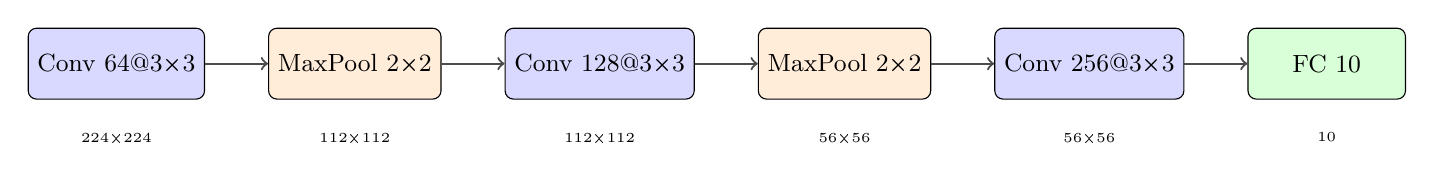
\begin{tikzpicture}[
    node distance=0.8cm,
    font=\small,
    % Node styles
    conv/.style={draw, rounded corners=3pt, minimum width=2cm, minimum height=0.9cm, fill=blue!15},
    pool/.style={draw, rounded corners=3pt, minimum width=2cm, minimum height=0.9cm, fill=orange!15},
    fc/.style={draw, rounded corners=3pt, minimum width=2cm, minimum height=0.9cm, fill=green!15},
    arrow/.style={->, thick, draw=black!70},
]

    % CNN layers
    \node[conv] (conv1) {Conv 64@3×3};
    \node[pool, right=of conv1] (pool1) {MaxPool 2×2};
    \node[conv, right=of pool1] (conv2) {Conv 128@3×3};
    \node[pool, right=of conv2] (pool2) {MaxPool 2×2};
    \node[conv, right=of pool2] (conv3) {Conv 256@3×3};
    \node[fc, right=of conv3] (fc) {FC 10};
    
    % Connections
    \draw[arrow] (conv1) -- (pool1);
    \draw[arrow] (pool1) -- (conv2);
    \draw[arrow] (conv2) -- (pool2);
    \draw[arrow] (pool2) -- (conv3);
    \draw[arrow] (conv3) -- (fc);
    
    % Dimension annotations
    \node[below=0.3cm of conv1, font=\tiny] {224×224};
    \node[below=0.3cm of pool1, font=\tiny] {112×112};
    \node[below=0.3cm of conv2, font=\tiny] {112×112};
    \node[below=0.3cm of pool2, font=\tiny] {56×56};
    \node[below=0.3cm of conv3, font=\tiny] {56×56};
    \node[below=0.3cm of fc, font=\tiny] {10};

\end{tikzpicture}
\end{document}
